\documentclass[10pt, landscape, a4paper]{article}
\usepackage{geometry}[landscape]
\usepackage{multicol}
\usepackage{graphicx}
\usepackage{amsmath} 
\usepackage{amssymb}
\usepackage{ccicons}
\usepackage{hyperref}


\usepackage[boxruled, linesnumbered]{algorithm2e}

%% This declares a command \Comment
\SetKwComment{Comment}{/* }{ */}

\usepackage[dvipsnames]{xcolor}

% Set page margins
\geometry{top=.8cm, left=.8cm, right=.8cm, bottom=.8cm}

% Set paragraph indentation
\setlength{\parindent}{0pt}

% Set path for assets
\graphicspath{{assets/}}

\setlength{\columnsep}{20pt}
\raggedcolumns

% _____ CUSTOM COMMANDS __________________________________________
\newcommand{\E}[0]{\mathbb{E}}
\newcommand{\R}[0]{\mathbb{R}}

\newcommand{\sgn}[0]{\text{sgn}}

\newcommand{\argmin}[1]{\underset{#1}{\text{argmin}}}
\newcommand{\argmax}[1]{\underset{#1}{\text{argmax}}}

\begin{document}
\begin{multicols*}{3}

% _____ CONTENT __________________________________________________

% main heading
\begin{center}
	\Large{\textbf{Computer Systems}} \\
    \small{by dcamenisch}
\end{center}

\section{Introduction}

This document is a summary of the 2022 edition of the lecture \textit{Computer Systems} at ETH Zurich. I do not guarantee correctness or completeness, nor is this document endorsed by the lecturers. If you spot any mistakes or find other improvements, feel free to open a pull request at \url{https://github.com/DannyCamenisch/systems-summary}. This work is published as CC BY-NC-SA.

\begin{center}
	\ccbyncsa
\end{center}
\section{Naming}

Naming is a fundamental concept, it allows resources to be bound at different times. Names are bound to objects, this is always relative to a context. One example of this would be path names, e.g. \textit{/usr/bin/emacs}. Name resolution can be seen as a function from context and name to some object. The resolved object can be a context in itself. This gives us a naming network.
\begin{center}
	\includegraphics[width=0.8\linewidth]{naming-network.png}
\end{center}

Both synonyms (two names bound to the same object) and homonyms (the same name bound to two different objects) can occur.
\section{The Kernel}

There are three main functions to an OS. Commonly they are referred to from a designer's view, but the user's view can be much more helpful to actually understand how it works.

\begin{center}
	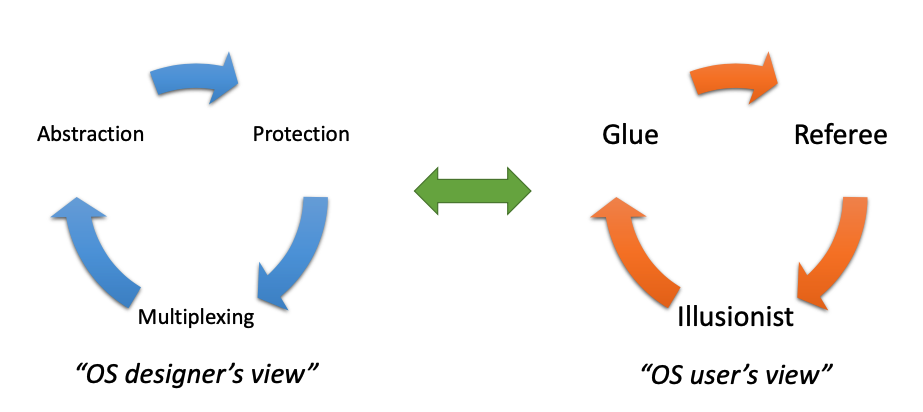
\includegraphics[width=\linewidth]{os-functions.png}
\end{center}


\subsection{Bootstrapping}

The term bootstrapping refers to pulling himself up from his own boots. In computer systems it is what we call the process of starting up a computer (booting). This boot process looks like this:

\begin{enumerate}
	\item CPU starts executing code at a fixed address (Boot ROM)
	\item Boot ROM code loads 2nd stage boot loader into RAM
	\item Boot loader loads kernel and optionally initials file system into RAM
	\item Jumps to kernel entry point
\end{enumerate}

The first few lines are always written in assembly, but generally we want to switch to C as soon as possible.


\subsection{Mode Switch}

One of our main goals is to protect the OS from applications that could harm it (intentionally or not). For this purpose we introduce two different modes:

\begin{itemize}
	\item \textbf{Kernel Mode} - execution with full privileges, read/write to any memory, access and I/O, etc. Code here must be carefully written
	\item \textbf{User Mode} - limited privileges, only those granted by the OS kernel
\end{itemize}

These two (or more) modes are already implemented in hardware. The main reason for a mode switch is when we encounter a processor exception (mode switch from user to kernel mode). If this is the case, we want the following to happen:

\begin{enumerate}
	\item Finish executing current instruction
	\item Switch mode from user to kernel
	\item Look up exception cause in exception vector table
	\item Jump to this address
\end{enumerate}

Further we may also want to save the registers and switch page tables. When switching between the modes we also have to change our address space, but we might want to access some informations from the user mode address space. One way of doing this is to use a so called \textbf{trampoline}, which is a part of the address space that gets mapped to the same location in user and kernel mode.

\begin{center}
	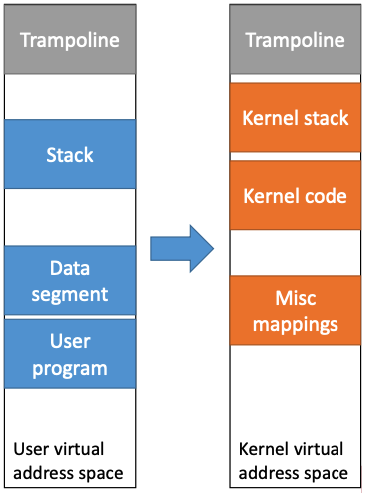
\includegraphics[width=0.4\linewidth]{trampoline.png}
\end{center}

Mode switches can also occur the other way around (from kernel mode to user mode). The main reasons for this are:

\begin{itemize}
	\item New process / thread start
	\item Return from exception
	\item Process / thread context switch
	\item User-level upcall (UNIX signal)
\end{itemize}

This leads us to the following perspective:

\begin{center}
	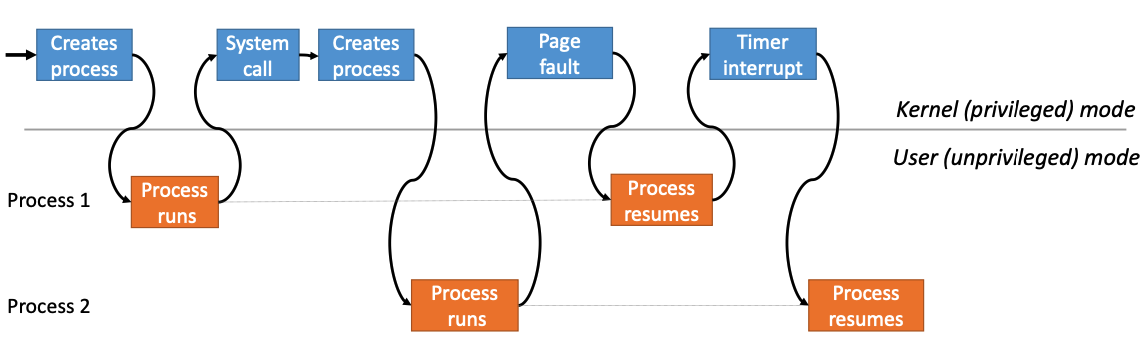
\includegraphics[width=\linewidth]{mode-switch.png}
\end{center}

The mode switch is fundamental to modern computers:

\begin{itemize}
	\item It enables virtualization of the processor
	\item It creates the illusion of multiple computers
	\item It referees access to the CPU
\end{itemize}


\subsection{General Model of OS Structure}

\begin{center}
	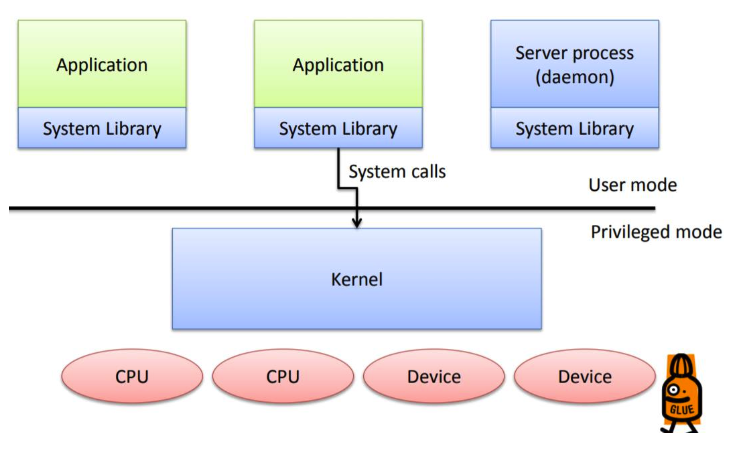
\includegraphics[width=0.9\linewidth]{os-structure.png}
\end{center}

\begin{itemize}
	\item \textbf{Kernel}: The kernel consists of software run in privileged mode. There might be more than one kernel in an OS. It can handle system calls, h/w interrupts etc.
	\item \textbf{System Libraries}: They are part of any application run on the machine and should provide an interface for the kernel.
	\item \textbf{Daemon}: This is a process running as part of the OS. It’s not run in privileged mode and may use system libraries. An example might be a file system.
\end{itemize}

We can differentiate between monolithic kernels and microkernels, depending on the amount of code in kernel mode.


\subsection{System Calls}

System calls are the only way for user mode programs to enter kernel mode. System calls are a type of exception, but they try to look a lot more like a procedure call. Therefore the kernel system call handler has to first locate arguments, copy these arguments into kernel memory, validate these arguments and then copy the results back into user memory after execution. An example of such a system call would be \textit{write()}. 


\subsection{Hardware Timers}

What happens if a user mode program does not cause any exception and does not give control back to the kernel? Hardware timers are a solution for this problem, the hardware device periodically interrupts the processor and returns control to the kernel handler, which sets the time of the next interrupt.

\section{Processes}

When you run a program, the OS creates a process to execute the program in. A process is an illusion created by the OS, it creates an execution environment for a program. This environment gives the program limited rights (access, name spaces, threads, etc.) and therefore it is both a security and a resource principal.


\subsection{Creating a Process}

There are two main approaches to creating new processes:

\begin{itemize}
	\item \textbf{Spawn} - constructs a running process from scratch
	\item \textbf{Fork / Exec} - creates a copy of the calling process or replaces the current program with another in the same process
\end{itemize}

\textbf{Spawn}

\begin{itemize}
	\item Create and initialize the process control block (PCB) in the kernel
	\item Create and initialize a new address space
	\item Load the program into the address space
	\item Copy arguments into memory in the address space
	\item Initialize the hardware context to start execution at "start"
	\item Inform the scheduler that the new process is ready to run
\end{itemize}

Spawn is very complex, we have to specify everything about the new environment. If we omit a key argument a new process might have insufficient rights or resources or it might fail to function due to a security fault. \medskip

\textbf{Fork}

Fork on the other hand is less complex. The child process is almost an exact copy of the parent, with a different PID. We know which process we are in from the return value of the \textit{fork()} call ($0$ for child, $>0$ for parent, $<0$ for error). The complete UNIX process management API also includes:

\begin{itemize}
	\item \textit{exec()} - system call to change the program being run by the current process
	\item \textit{wait()} - system call to wait for a process to finish
	\item \textit{signal()} - system call to send a notification to another process
\end{itemize}

In contrast to \textit{spawn()}, here the child revokes rights and access explicitly before \textit{exec()}, further we can use the full kernel API to customize the execution environment.


\subsection{The Process Control Block}

The PCB is the main kernel data structure used to represent a process. It has to hold or refer to the page table, trap frame, kernel stack, open files, program name, scheduling state, PID, etc.


\subsection{Process Context Switching}

Context switching is the process of switching between different processes running in user mode or kernel mode. It is one of the key elements of the illusion that multiple programs can run in parallel. \columnbreak

There are two main reasons for the kernel to switch processes: either when a process has run for too long and gets interrupted by a hardware timer or when a process blocks. The second case happens when a system call can not complete immediately. The process then often calls \textit{sleep()} and other processes can be executed.
\begin{center}
	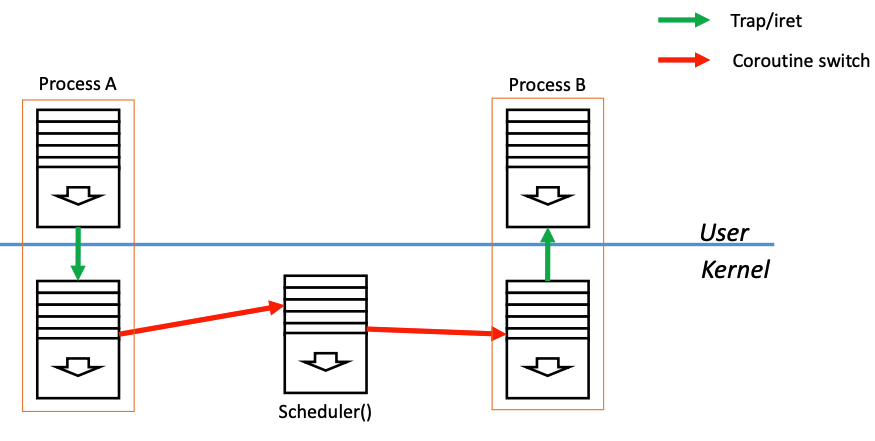
\includegraphics[width=\linewidth]{context-switching.png}
\end{center}


\subsection{Process Hierarchy}

By forking and spawning new processes we create sort of a hierarchy. If a child process dies, but the parent does not call \textit{wait()}, the child process becomes a zombie - it is dead, but still around since nobody asked for the return code. If a parent dies, but the child does not, the child becomes an orphan and gets reparented to the first process (PID \#1, \textit{init}).
\begin{center}
	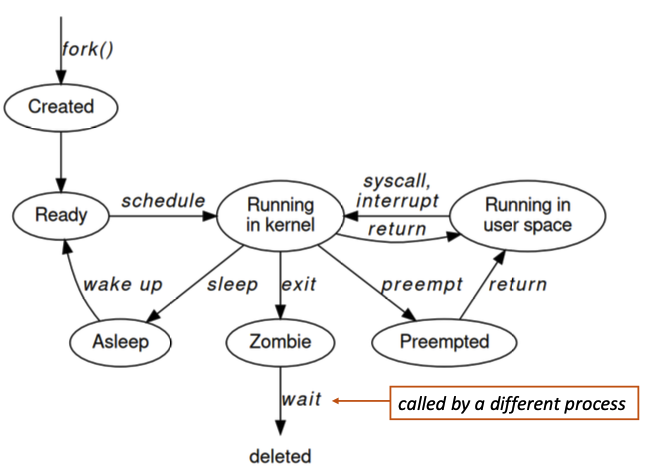
\includegraphics[width=\linewidth]{process-life-cycle.png}
\end{center}

The \textit{init} process is basically an infinite loop calling \textit{wait}(NULL), it gets rid of any zombies.


\subsection{Threads}

Threads are used as an abstraction for concurrency. They allow the usage of parallel hardware, e.g. multiple cores. A thread basically consist of a stack and some register values.\medskip

There is a distinction between \textbf{user threads} and \textbf{kernel threads}. The former are implemented entirely in user’s process. If a user thread is about to block (e.g. when executing a system call), the thread library usually interrupts this call and does something non blocking instead while the system call is served. Kernel threads are implemented by the OS kernel directly. They thus appear as different virtual processors to the user process. In this model, a set of threads share a virtual address space together. Each thread is now scheduled by the kernel itself, which keeps track of threads are part of which process. However, this makes the kernel more complicated.

\section{Inter-Process Communication}

It is often the case, that we want different processes to work together, e.g. DB and web-scraper. For this we need ways to exchange information between processes, we call this inter-process communication or IPC.\medskip

One of the most basic ways to exchange information is system calls. We save our data on the stack or in a register and execute the system call, the kernel then switches execution to the other process with the information about the data that should be exchanged. This is a really flawed approach some reasons are that context switches are expensive and it is unsafe to introduce new system calls for each task.

\subsection{Shared Memory}

We introduce shared memory that can only be accessed by the processes that communicate with each other. This requires us to define a common interface between the processes. The main building blocks for this are:
\begin{itemize}
	\item Shared area: registers, memory - define the layout of the memory
	\item Indicating status: shared variables, signals
	\item Updating status: changing variables
	\item Consistency: use synchronization primitives
\end{itemize}

When checking the state of a shared variable polling can be very inefficient. As an alternative we can use a signal handler. When the first process calls the signal handler, the kernel notifies the second process of the update. When the kernel issues such a system call to a process, we call it an \textbf{upcall}. To guarantee consistency, we use synchronization primitives that are already known from previous lectures (spin locks with CAS, TAS, etc.). \medskip

A more modern approach is to use transactional memory, hereby we work with transactions that can fail on race condition.

\section{Scheduling}

First we introduce some terminology, notice how the wait time is defined as the combination of hold time and execution time.
\begin{center}
	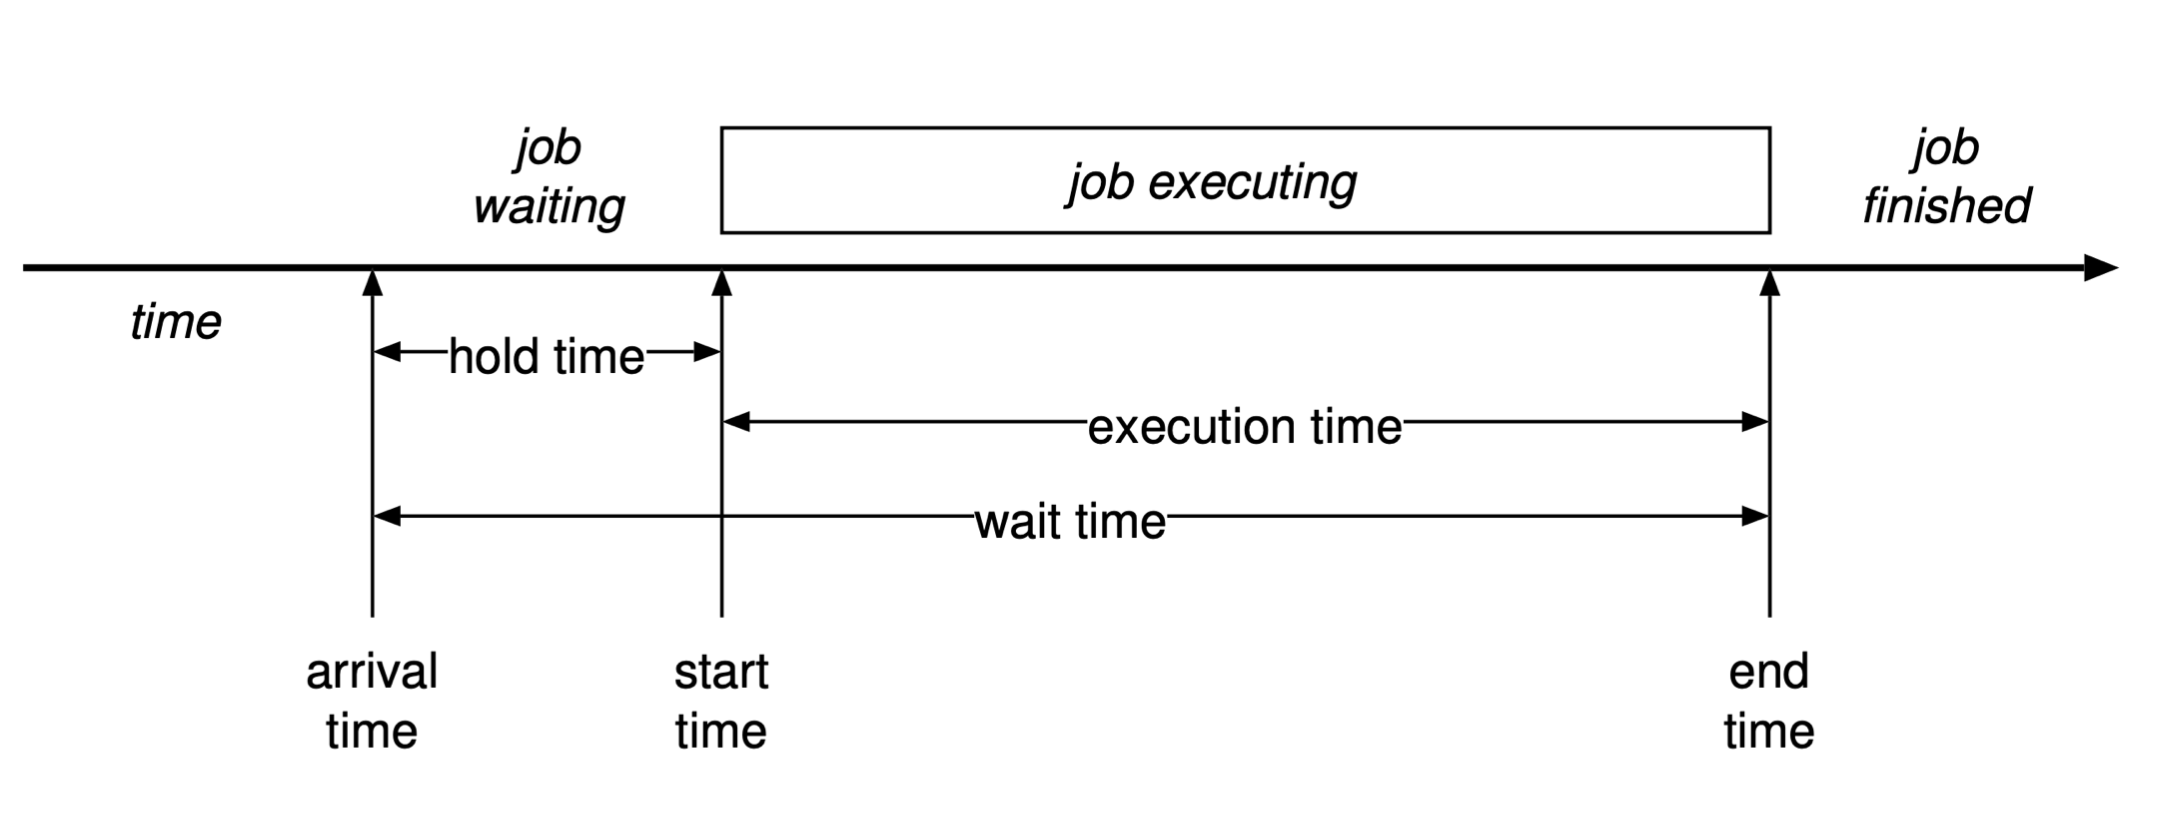
\includegraphics[width=\linewidth]{scheduling.png}
\end{center}

The important metrics for scheduling are throughput (rate of completing jobs) and overhead (time spent without a job executing).

In the following part we will look at various scheduling algorithms, starting from a very simple approach.

\subsection{Non-Preemptive Batch Oriented}

There are two basic algorithms:
\begin{itemize}
	\item First Come First Served
	\item Shortest Job First
\end{itemize}

Both are algorithms are very simple to implement but their applications are limited.

\subsection{Preemptive Batch Oriented}

We introduce preemption, meaning that we interrupt the execution after some finite time interval. After such an interrupt we decide which program to run next. \smallskip

\textbf{Modified SJF:} Go through the sorted list of jobs and execute each until interrupted. Note that the length of a job does not get recomputed after an execution. \smallskip

\subsection{Interactive Scheduling}

When running interactive workload, we can encounter events that block the execution (I/O, page-faults, etc.). During this time we would like to run another program instead of wasting execution time. \smallskip

\textbf{Round Robin Scheduling:} Let $R$ be a queue and $q$ be the scheduling quantum:
\begin{enumerate}
	\item Set an interval timer for an interrupt $q$ seconds in the future
	\item Dispatch the job at the head of $R$
	\item If blocking happens or the timer runs out, return to the scheduler
	\item Push the previously running job to the tail of $R$
\end{enumerate}

\textbf{Priority Based Scheduling:} We assign a priority to each task and dispatch the highest priority task first, if we have ties we use RR to break them. To avoid starvation we might want to use dynamic priorities (increased priority depending on wait time). An even more complex approach is to introduce multi-level queues, meaning that we have a fixed number of queues that assign priorities within each queue. Then we use RR scheduling between the queues to execute tasks. \medskip

Priority scheduling runs into problems when a high priority process has to wait for a lock from a low priority process (Priority Inversion). To fix this, we can either introduce inheritance - the holder of the lock acquires the priority of the highest waiting process - or ceiling - the holder of the lock runs at the highest priority.

\subsection{Linux o(1) Scheduler}

Linux uses 140 multilevel feedback queues, each with a different priority. Multilevel feedback queues penalize CPU bound tasks and prioritize I/O operations, as I/O tasks will eventually block.

The priority range 0-99 is used for high priority, static tasks and it uses FCFS or RR scheduling. The range 100-139 is for user tasks and uses RR together with priority ageing for I/O tasks.


\section{Input / Output}

Every OS has an I/O subsystem, which handles all interaction between the machine and the outside world. The I/O subsystem abstracts individual hardware devices to present a more or less uniform interface, provides a way to name I/O devices, schedules I/O operations and integrates them with the rest of the system, and contains the low-level code to interface with individual hardware devices. \medskip

To an OS programmer, a \textbf{device} is a piece of hardware visible from software. It typically occupies some location on a bus or I/O interconnect, and exposes a set of hardware registers which are either memory mapped or in I/O space. A device is also usually a source of interrupts, and may initiate Direct Memory Access (DMA) transfers. \medskip

The \textbf{device driver} for a particular device is the software in the OS which understands the specific register and descriptor formats, interrupt models, and internal state machines of a given device and abstracts this to the rest of the OS.

\subsection{Data Transfer}

\textbf {Programmed I/O} consists of causing input/output to occur by reading/writing data values to hardware registers. This is the simples form of communication. It is fully synchronous, so the CPU always has to be involved. Further it is polled, the device has no way to signal that new data is ready. \medskip

\textbf{Interrupts} can be used to signal the availability of new data and solve the polling problem. But the problem of CPU involvement still persists.
\begin{center}
	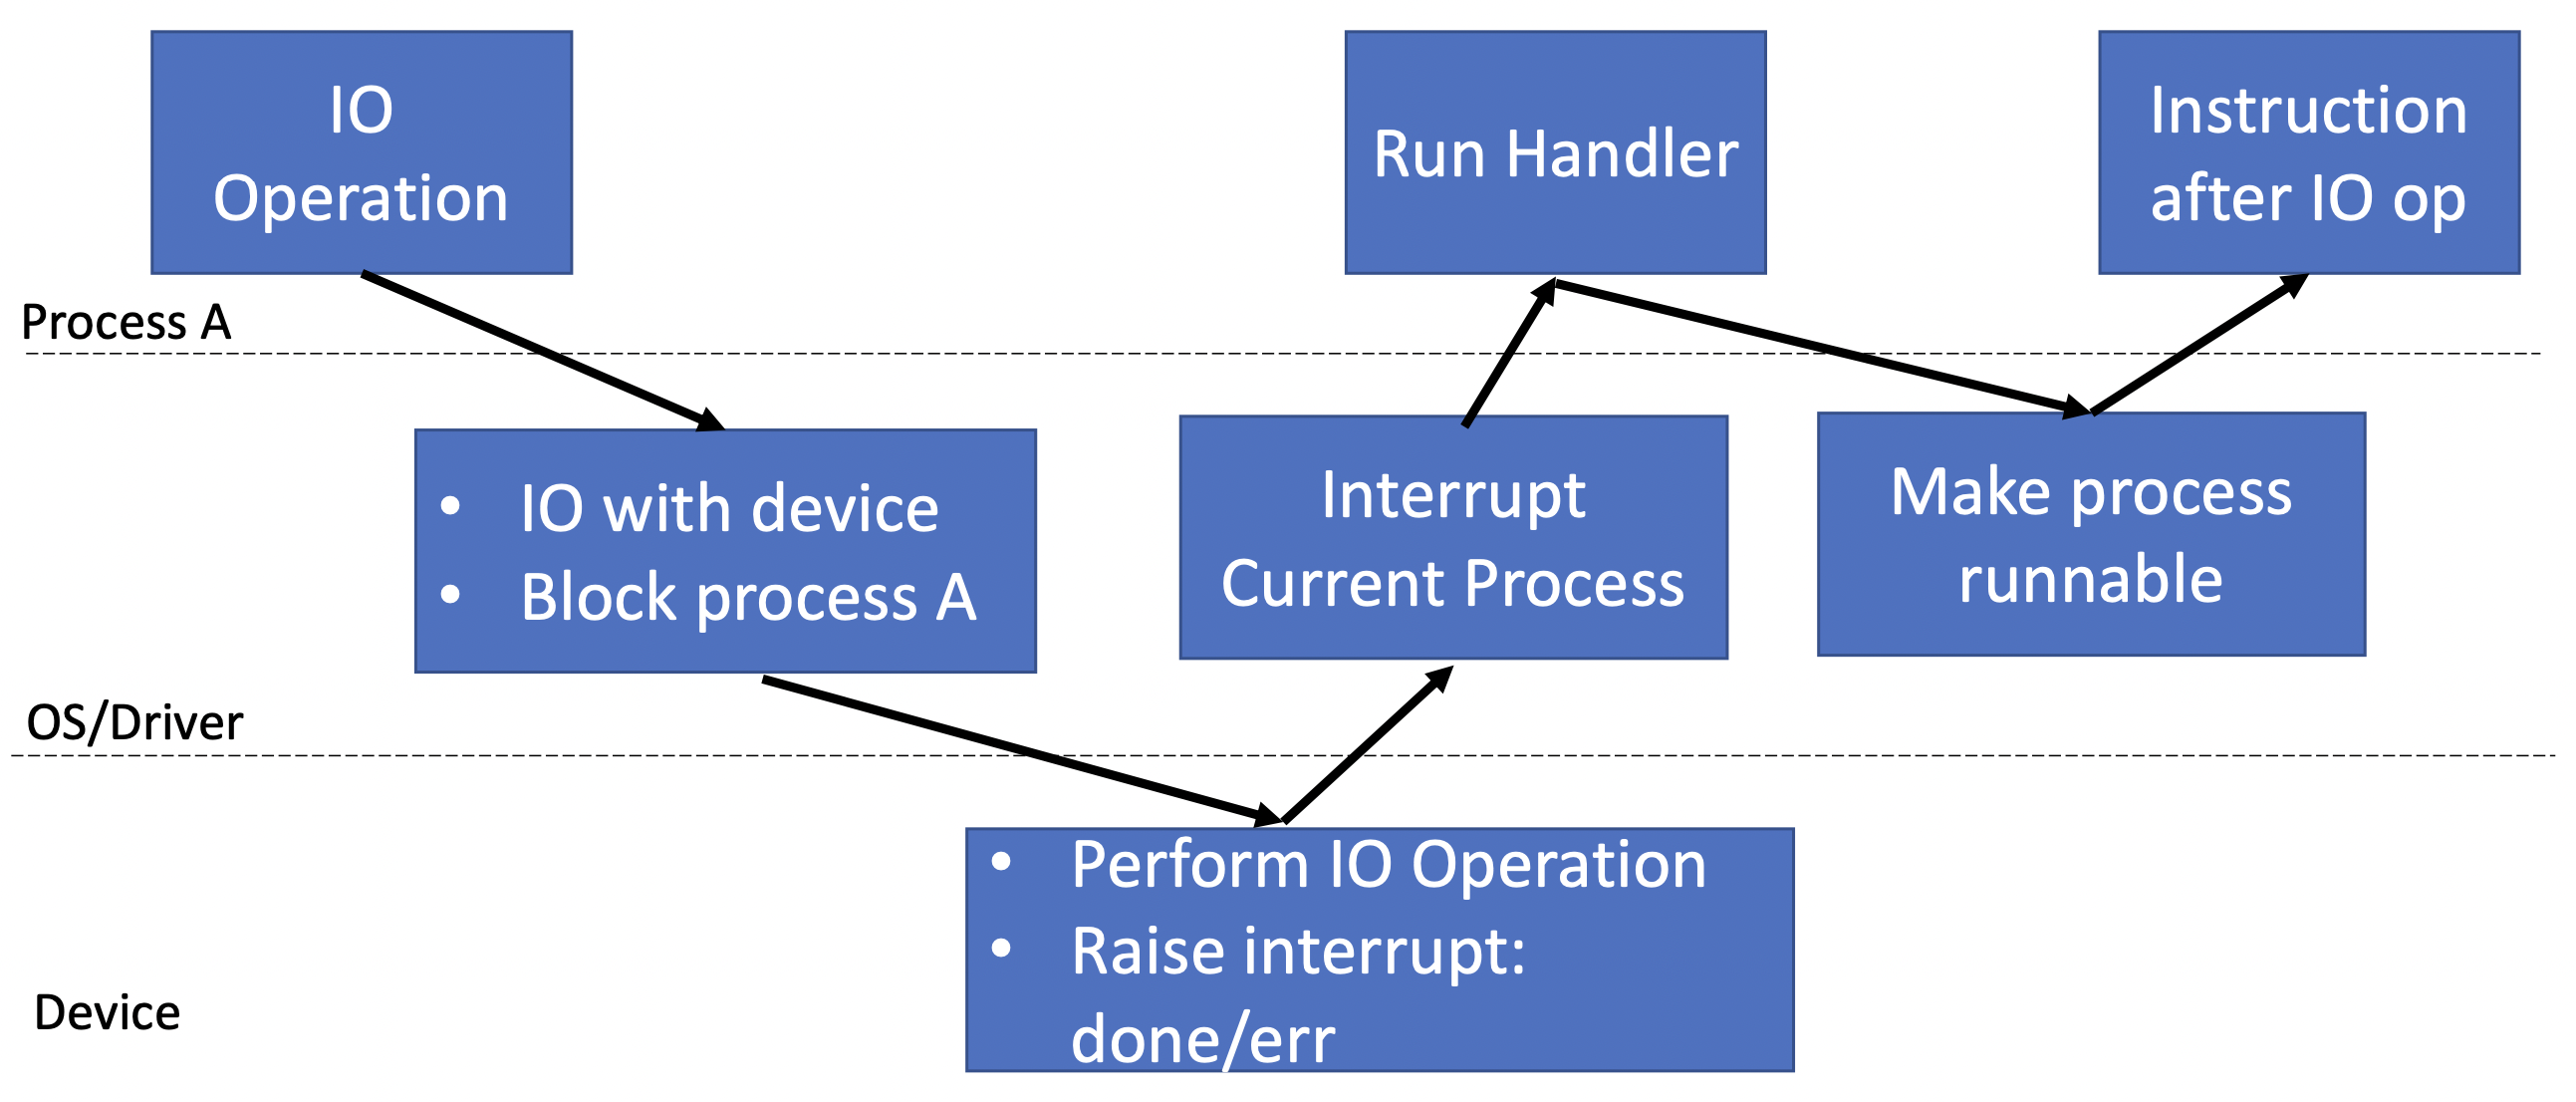
\includegraphics[width=\linewidth]{data_transfer_interrupt.png}
\end{center}

\textbf{Direct Memory Access} or DMA, a device can be given a pointer to buffers in main memory and transfer data to and from those buffers without further involvement from the CPU. A single interrupt is used to signal the end of data transfer. DMA is, for the most part, physical (not virtual) access to memory. Further DMA transfers to and from main memory may or may not be coherent with processor caches.

\subsection{Asynchrony}

Device drivers have to deal with the fundamentally asynchronous nature of I/O: the system must respond to unexpected I/O events, or to events which it knows are going to happen, but not when. \medskip

The \textbf{First-level Interrupt Service Routine} (FLISR) is the code that executes immediately as a result of the interrupt. It runs regardless of what else is happening in the kernel. As a result, it can't change much since the normal kernel invariants might not hold. \medskip

Since I/O is for the most part interrupt-driven, but data is transferred to and from processes which perform explicit operations to send and receive it. Consequently, data must be buffered between the process and the interrupt handler, and the two must somehow rendezvous to exchange data. There are three canonical solutions to this problem:

A \textbf{deferred procedure call}, is a program closure created by the 1st-level interrupt handler. It is run later by any convenient process, typically just before the kernel is exited. \medskip

A \textbf{driver thread}, sometimes called an interrupt handler thread, serves as an intermediary between ISR and processes. The thread starts blocked waiting for a signal either from the user process or the ISR. When an interrupt occurs or a user process issues a request, the thread is unblocked (this operation can be done inside an ISR) and it performs whatever I/O processing is necessary before going back to sleep. Driver threads are heavyweight: even if they only run in the kernel, the still require a stack and a context switch to and from them to perform any I/O requests. \medskip

The third alternative, is to have the FLISR convert the interrupt into a message to be sent to the driver process. This is conceptually similar to a DPC, but is even simpler: it simply directs the process to look at the device. However, it does require the FLISR to synthesize an IPC message, which might be expensive. In non-preemptive kernels which only process exceptions serially, however, this is not a problem, since the kernel does not need locks. \medskip

\textbf{Bottom-half handler} - the part of a device driver code which executes either in the interrupt context or as a result of the interrupt. \medskip

\textbf{Top-half handler} - the part of a device driver which is called "from above", i.e. from user or OS processes.

\subsection{Device Models}

The device model of an OS is the set of key abstractions that define how devices are represented to the rest of the system by their individual drivers. It includes the basic API to a device driver, but goes beyond this: it encompasses how devices are named throughout the system, and how their interconnections are represented as well. \medskip

\textbf{UNIX device model:}
\begin{itemize}
	\item Character Devices - used for unstructured I/O and present a byte-stream interface with no block boundaries.
	\item Block Devices - used for structured I/O and deal with blocks of data at a time.
	\item Network Devices - correspond to a network interface adapter. It is accessed through a rather different API.
	\item Pseudo Devices - a software service provided by the OS kernel which it is convenient to abstract as a device, even though it does not correspond a physical piece of hardware.
\end{itemize}

\subsection{Protection}

Another function of the I/O subsystem is to perform protection. Ensuring that only authorized processes can access devices or services offered by the device driver and that a device can't be configured to do something harmful. Unix controls access to the drivers themselves by representing them as files, and thereby leveraging the protection model of the file system. DMA-capable devices are in principle capable of writing to physical memory anywhere in the system, and so it is important to check any addresses passed to them by the device driver. Even if you trust the driver, it has to make sure that it’s not going to ask the device to DMA somewhere it shouldn’t. One approach is to put a memory management unit (MMU) on the path between the device and main memory, in addition to each core having one.

\section{Virtual Memory}

From previous courses we know MMUs, TLBs and basic paged virtual memory operations. The uses for address translation include: Process Isolation, Shared Code Segments, Dynamic Memory Allocation and many more.


\subsection{Segments}

Before paging, there were segments. Before segments there where base and limit registers. These contained two addresses $B$ and $L$. A CPU access to an address $a$ is permitted iff $B \leq a < L$. Relocation registers are an enhanced form of base register. All CPU accesses are relocated by adding the offset: a CPU access to an address $a$ is translated to $B + a$. This allows each program to be compiled to run at the same address (e.g. 0x0000). \medskip
\begin{center}
	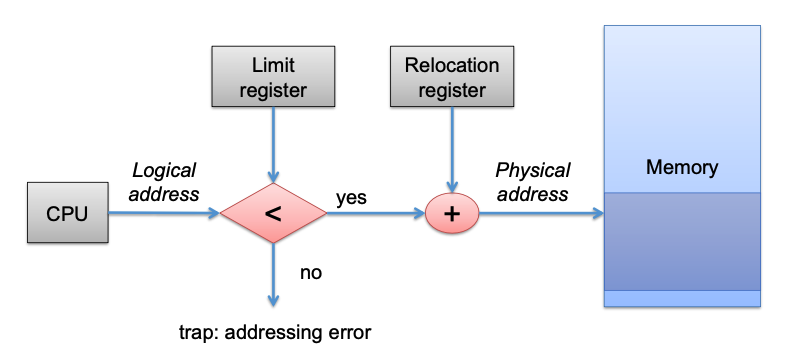
\includegraphics[width=\linewidth]{base-relocation-register.png}
\end{center}

A segment is a triple $(I, B_I, L_I)$ of values specifying a contiguous region of memory address space with base $B_I$, limit $L_I$, and an associated segment identifier $I$ which names the segment. Memory in a segmented system uses a form of logical addressing: each address is a pair $(I, O)$ of segment identifier and offset. A Segment Table is an in-memory array of base and limit values $(B_I, L_I)$ indexed by segment identifier, and possibly with additional protection information.
\begin{center}
	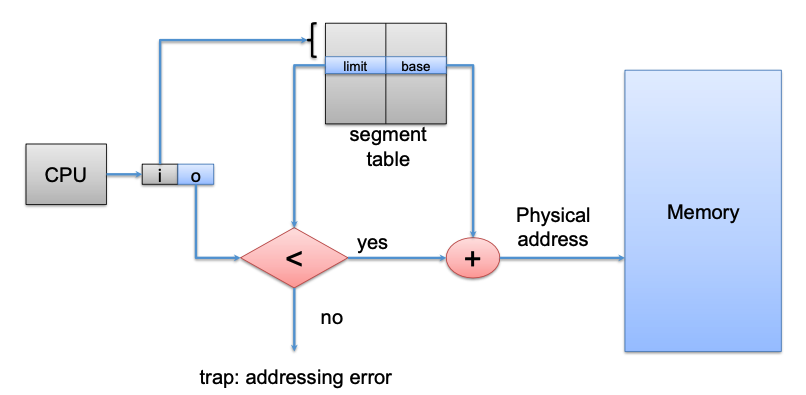
\includegraphics[width=\linewidth]{segment.png}
\end{center}

This enables sharing code/data segments between processes, further it adds protection and allows transparently growing stack/heap as needed. The principal downside of segmentation is that segments are still contiguous in physical memory, which leads to external fragmentation.


\subsection{Paging}

This is a short recap of paging. Virtual memory is divided into (virtual) pages of the same size having a VPN, physical memory gets divided into frames / physical pages having a PFN / PPN. Then a page table gets used to map VPNs to PFNs. This is implemented in hardware as the MMU. To speed up translation the TLB is used. Getting data from memory can work as follows (in this case we have a TLB miss):
\begin{center}
	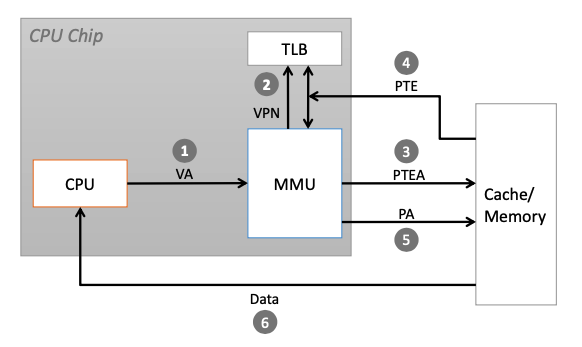
\includegraphics[width=\linewidth]{tlb-miss.png}
\end{center}

We have also seen how multi-level page tables work. Multi-level translation allows us to allocate only page table entries that are in use and makes memory allocation simpler.
\begin{center}
	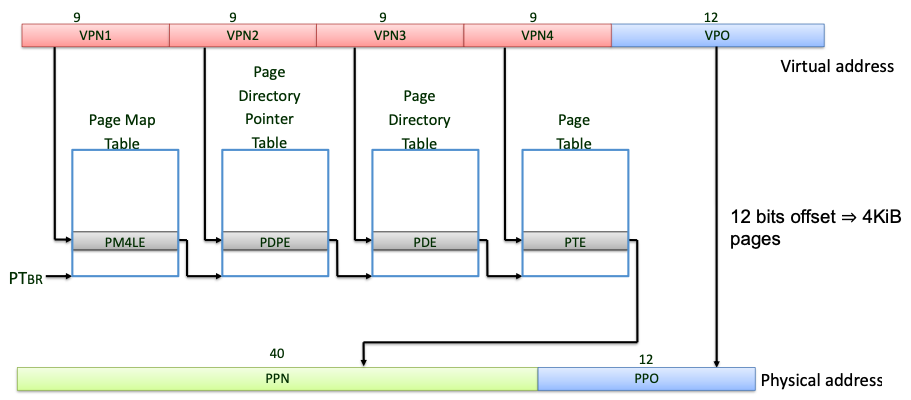
\includegraphics[width=\linewidth]{multi-level-pt.png}
\end{center}

On a context switch we need to store/restore the pointer to the page table and its size. One of the downsides of paging is if our page is very small and we do not need all of the space, this leads to internal fragmentation.


\subsection{Paged Segmentation}

It is possible to combine segmentation and paging. A paged segmentation memory management scheme is one where memory is addressed by a pair (segment.id, offset), as in a segmentation scheme, but each segment is itself composed of fixed-size pages whose page numbers are then translated to physical page numbers by a paged MMU.
\begin{center}
	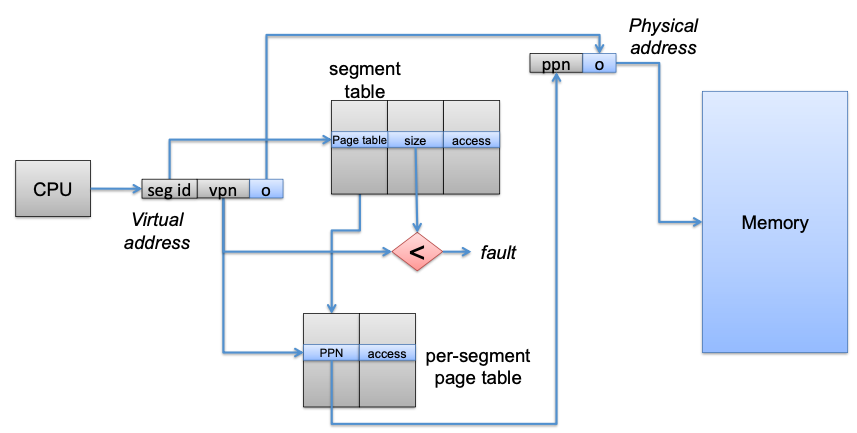
\includegraphics[width=\linewidth]{paged-segments.png}
\end{center}

One of the main benefits here is that each segment can have its own size of page table.


\subsection{Zero-on Reference}

The question how much physical memory is needed, is difficult to answer. So when a program runs out of memory, the system does the following:
\begin{enumerate}
	\item Page fault into OS kernel
	\item Kernel allocates some memory
	\item Zeroes the memory
	\item Modify page table
	\item Resume process
\end{enumerate}


\subsection{Fill On Demand}

Most programs do not need all their code to start running and might never use some code in its execution. Therefore we want to do something similar, we want to start a program before its code is in physical memory:
\begin{enumerate}
	\item Set all page table entries to invalid
	\item On first page reference, kernel trap
	\item Kernel brings page in from disk
	\item Resume execution
	\item Remaining pages can be transferred in the background while the program is running
\end{enumerate}


\subsection{Copy On Write}

Remember that we said \textit{fork()} copies the entire address space. This can be expensive and might not feasible in performance. On \textit{fork()} we copy the page table and set all mappings to read-only in both address spaces. Reads are now possible for both processes. If a write in either process causes a protection fault the kernel allocates a new frame and copies the referenced frames content into it. The faulting process now maps to the new copy and the protection changes to read/write (also for the non-faulting process).


\subsection{Managing Caches and the TLB}

\subsubsection{TLBs}

A problem with TLBs on context switches is that they can hold content inaccessible to the new process. To avoid having to flush the TLB, we introduce tags. Each TLB entry has a $6$-bit tag and the OS keeps track of a mapping between processes and tags. \medskip

\subsubsection{Caches}

\begin{center}
	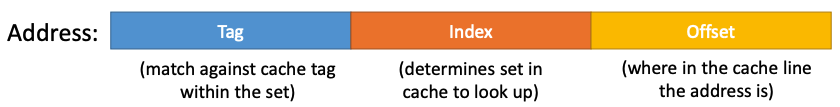
\includegraphics[width=\linewidth]{address.png}
\end{center}

Remember the different types of caches:
\begin{itemize}
	\item Virtually indexed, virtually tagged - simple and fast, but context switches are hard
	\item Physically indexed, physically tagged - can only be accessed after address translation
	\item Virtually indexed, physically tagged - overlap cache and TLB lookups
	\item Physically indexed, virtually tagged
\end{itemize}

Also remember the different write (write through, write back) and allocate (write allocate, non-write allocate) policies. In virtually tagged caches we can encounter homonyms, the same virtual address maps to multiple physical address spaces. To avoid this we can use physical tags, add address space identifiers, try to ensure disjoint address spaces or flush the cache on a context switch. \medskip

There is also a synonyms problem, where two virtual addresses map to the same physical address. This leads to inconsistent cache entries. The solutions to the homonym problem do not help here. To solve this problem we restrict VM mappings, so that synonyms map to the same cache set. 


\subsection{Demand Paging}

Demand paging solves the problem how to find a frame to use for missing pages. The goal is to minimize the page fault rate $p$ ($0 \leq p \leq 1$). The metric we are interested in is the effective access time $(1-p) * l_m + p * l_f$, where $l_m$ is the latency of a memory access and $l_p$ the latency of a page fault handling. Generally speaking the performance of a paging system depends on how many frames it has, but there is a diminishing return on adding new frames.

\subsubsection{Page Replacement Policies}

If a page has to be evicted, which one should be choose? We have already seen Least Recently Used (LRU) and First In First Out (FIFO). Both of these are not optimal, LRU is too expensive and FIFA works poorly for most workloads. A good compromise is the \textbf{Clock} or \textbf{2nd Chance} algorithm. It approximates LRU but much cheaper. It requires a linear table of all PFNs, with associated referenced bits. This can be best visualized as a circular buffer.
\begin{center}
	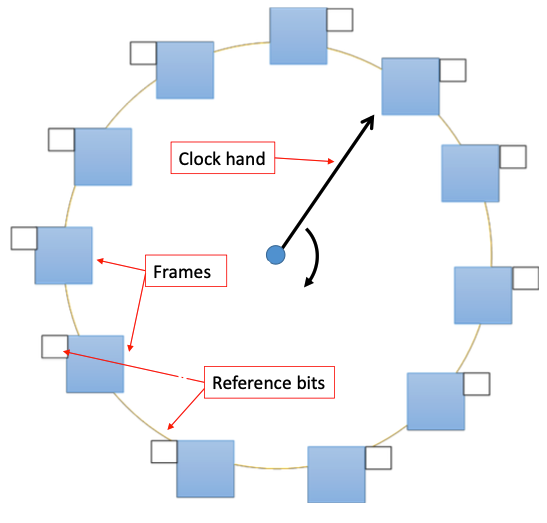
\includegraphics[width=0.8\linewidth]{2nd.png}
\end{center}

It works as follows:
\begin{itemize}
	\item Mark each frame when referenced for the first time
	\item If we want to replace a frame, process as follows: 
		\begin{itemize}
			\item If marked, unmark and advance the clock hand
			\item If unmarked, allocate this frame and mark it
		\end{itemize}
\end{itemize}

\subsubsection{Frame States}

\begin{center}
	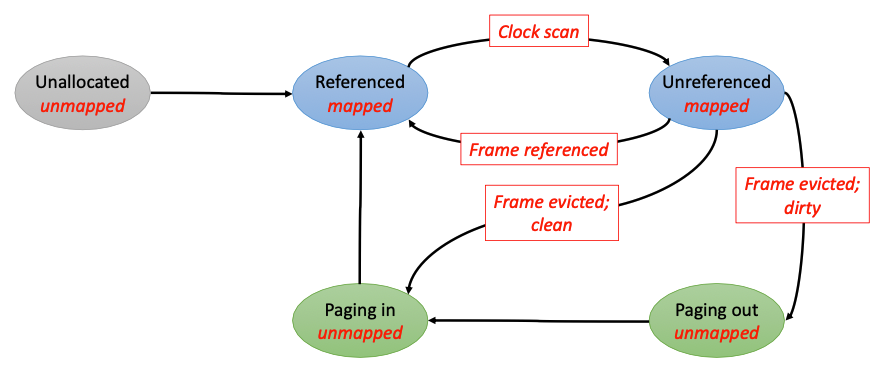
\includegraphics[width=\linewidth]{state_machine.png}
\end{center}

This only works if the corresponding bits are present in the page table and are properly set, in RISC-V for example these bits are present but do not have to be set. We can emulate these bits using faults.


\begin{center}
	\Large{\textbf{Distributed Systems}}
\end{center}

Today almost all computer systems are distributed, for different reasons:
\begin{itemize}
	\item Geography
	\item Parallelism - speed up computation
	\item Reliability - prevent data loss
	\item Availability - allow for access at any time, without bottlenecks, minimizing latency
\end{itemize}

Even though distributed systems have many benefits, such as increased storage or computational power, they also introduce challenging coordination problems.
\section{Fault Tolerance and Paxos}

In this section we want to create a fault-tolerant distributed system. We start out with a simple approach and improve our solution until we arrive at a system that works even under adverse circumstance, Paxos. \medskip

A \textbf{node} is a single actor in the system. In the message passing model we study distributed systems that consist of a set of nodes, where each node can perform local computations and send messages to every other node. Message loss means that there is no guarantee that a message will arrive safely at the receiver. This leads us to the first algorithm \medskip

\begin{algorithm}[H]
\caption{Naive Client-Server Algorithm}
	Client sends commands one at a time to server\\
	Server acknowledges every command\\
	If the client does not receive an acknowledgment within a reasonable time, it resends the command
\end{algorithm}

\medskip

This simple algorithm is the basis of many reliable protocols, e.g. TCP. The algorithm can easily be extended to work with multiple servers: The client sends each command to every server, and once the client received an acknowledgment from each server, the command is considered to be executed successfully. \medskip

In practice, messages might experience different transmission times, even if they are being sent between the same two nodes. A set of nodes achieves \textbf{state replication}, if all nodes execute a sequence of commands in the same order. Since state replication is trivial with a single server, we can desig- nate a single server as a serializer. \medskip

\begin{algorithm}[H]
\caption{State Replication with a Serializer}
	Client sends commands one at a time to the serializer\\
	Serializer forwards commands one at a time to all other servers\\
	Once the serializer received all acknowledgments, it notifies the client about the success
\end{algorithm}

\medskip

The downside of this algorithm is that the serializer is a single point of failure.

\subsection{Two-Phase Protocol}

\begin{algorithm}[H]
\caption{Two-Phase Protocol}
	\Comment{Phase 1}
	Client asks all servers for the lock \\
	\Comment{Phase 2}
	\eIf{client receives lock from every server}{
		Client sends command reliably to each server and gives the lock back
	}{
		Clients gives the received locks back \\
		Client waits, and then starts with Phase 1 again
	}
\end{algorithm}

\medskip

Instead of directly establishing a consistent order of commands, we can use a different approach: We make sure that there is always at most one client sending a command; i.e., we use mutual exclusion, respectively locking. \medskip

Still there are quite some problems with this algorithm. What happens if the node holding the locks crashes or it only gets part of the locks?

\subsection{Paxos}

A \textbf{ticket} is a weaker form of a lock, with the following properties:
\begin{itemize}
	\item Reissuable: A server can issue a ticket, even if previously issued tickets have not yet been returned.
	\item Ticket expiration: If a client sends a message to a server using a previously acquired ticket $t$, the server will only accept $t$, if it is the most recently issued ticket.
\end{itemize}

There is no more problem with crashes: If a client crashes while holding a ticket, the remaining clients are not affected. (At this point the naive ticket protocol is left out) \medskip

\begin{algorithm}[H]
\caption{Paxos Client / Proposer}
	\Comment{Initialization}
	$c$ 		\tcc*[f]{command to execute}\\
	$t = 0$ 	\tcc*[f]{ticket number to try}\\
	
	\BlankLine
	\Comment{Phase 1}
	$t = t + 1$\\
	Ask all servers for ticket $t$
	
	\BlankLine
	\Comment{Phase 2}
	\If{a majority answers ok}{
		Pick($T_{store}, C$) with largest $T_{store}$
		\If{$T_{store} > 0$}{
			$c = C$
		}
		Send propose($t, c$) to same majority
	}
	
	\BlankLine
	\Comment{Phase 3}
	\If{a majority answers success}{
		Send execute($c$) to every server
	}
\end{algorithm}

\medskip

\begin{algorithm}[H]
\caption{Paxos Server / Acceptor}
	\Comment{Initialization}
	$T_{max} = 0$ 	\tcc*[f]{largest issued ticket}\\
	$C = \bot$ 		\tcc*[f]{stored command}\\
	$T_{store} = 0$ 	\tcc*[f]{ticket used to store $C$}\\
	
	\BlankLine
	\Comment{Phase 1}
	\If{$t > T_{max}$}{
		$T_{max} = t$\\
		Answer with ok($T_{max}, C$)
	}
	
	\BlankLine
	\Comment{Phase 2}
	\If{$t = T_{max}$}{
		$C = c$\\
		$T_{store} = t$\\
		Answer success
	}
	
\end{algorithm}

\medskip

Unlike previously mentioned algorithms, there is no step where a client explicitly decides to start a new attempt and jumps back to Phase 1. This has the advantage that we do not need to be careful about selecting “good” values for timeouts, as correctness is independent of the decisions when to start new attempts. The performance can be improved by letting the servers send negative replies in Phase 1 or 2 if the ticket expired. Using randomized backoff we can eliminate contention between clients. \medskip

\textbf{Theorem:} If a command c is executed by some servers, all servers (eventually) execute c. \medskip

Note that Paxos cannot make progress if half (or more) of the servers crash, as clients cannot achieve a majority anymore. \medskip

For state replication we need to be able to execute multiple commands, we can extend each instance with an instance number, that is sent around with every message. Once the 1st command is chosen, any client can decide to start a new instance and compete for the 2nd command. If a server did not realize that the 1st instance already came to a decision, the server can ask other servers about the decisions to catch up.


\end{multicols*}
\end{document}

% ____ FOOTER ______________________________________________________
% Content and Template: 
% original by Danny Camenisch (dcamenisch@inf.ethz.ch), 2022
% based on different summaries from many helpful people